% !TEX program = xelatex
% Mixture-of-Memory 课程成果报告 — 编译: xelatex -> xelatex (跑两遍生成目录/引用)
% 或: latexmk -xelatex MoM_report.tex
\documentclass[11pt,a4paper]{ctexart}

\usepackage[margin=2.3cm,top=2.2cm,bottom=2.2cm]{geometry}
\usepackage{amsmath}
\usepackage{graphicx}
\usepackage{xcolor}
\usepackage{booktabs}
\usepackage{caption}
\usepackage{float}
\usepackage{enumitem}
\usepackage{fancyhdr}
\usepackage{titlesec}
\usepackage[hidelinks]{hyperref}
\usepackage{array}

% ---- 颜色 / 标题风格 ----
\definecolor{titleblue}{RGB}{20,40,90}
\definecolor{headgray}{RGB}{150,150,150}
\definecolor{rowblue}{RGB}{225,232,245}
\definecolor{rowgray}{RGB}{240,240,240}

\titleformat{\section}{\Large\bfseries\color{titleblue}}{\thesection}{0.6em}{}
\titleformat{\subsection}{\large\bfseries\color{titleblue}}{\thesubsection}{0.5em}{}
\titlespacing*{\section}{0pt}{1.2ex plus .2ex}{0.8ex}
\titlespacing*{\subsection}{0pt}{0.8ex}{0.5ex}

\setlist[itemize]{leftmargin=1.6em,topsep=2pt,itemsep=1.5pt,parsep=0pt}

% ---- 页眉页脚 ----
\pagestyle{fancy}
\fancyhf{}
\fancyhead[C]{\footnotesize\color{headgray} Mixture-of-Memory · 大模型驱动的软件开发 课程成果报告}
\fancyfoot[C]{\footnotesize\color{headgray} -\,\thepage\,-}
\renewcommand{\headrulewidth}{0pt}
\renewcommand{\footrulewidth}{0pt}

\captionsetup{font=small,labelfont=bf}

\begin{document}

% ================= 封面 =================
\thispagestyle{empty}
\begin{center}
  \vspace*{0.5cm}
  {\LARGE\bfseries\color{titleblue} Mixture-of-Memory：用固定大小记忆缓冲\\[2pt]
   压缩长上下文的 LLM 适配器\par}
  \vspace{0.4cm}
  {\large —— 一次由大模型 Agent 自主驱动的研发实践\par}
  \vspace{0.8cm}
  {\normalsize
   课程：大模型驱动的软件开发（2026 春季学期）成果报告\\[3pt]
   姓名：刘涵祚\qquad 班级：计科 41\\[3pt]
   源码：\url{https://github.com/liuhanzuo/Mixture-of-Memory}\par}
  \vspace{0.5cm}
  \rule{0.7\textwidth}{0.4pt}
\end{center}

\vspace{0.2cm}
\begin{center}{\large\bfseries\color{titleblue} 摘要}\end{center}
\noindent
本工作研究如何把超长上下文压缩进一个固定大小的记忆缓冲（memory bank），
使 Llama-3-8B 在有界 KV 预算下处理长序列。我们提出的 mem\_space 适配器与混合专家（MoE）
高度同构——可视为 \textbf{Mixture-of-Memory（MoM）}：$N$ 个记忆 slot 即“专家”，
一个轻量 selector 对每个 chunk 做 top-$k$ 路由，写入只更新被选中的 top-$k$ slot（稀疏更新），
读出则对全部 $N$ 个 slot 做独立 softmax。我们诊断出该架构的核心瓶颈是
\textbf{“写得进、读不准”}（纯记忆读出 W0 仅 10--30，而开卷上限 50--60），
并系统比较了四类干预：token-mass 读出加权、self-study 蒸馏、长度课程、以及二者叠加。
关键发现是\textbf{弱 mass（强度 $\approx0.5$）与蒸馏在长程（16k/32k）上首次产生协同}，
超过任一单独方法；mass 过强反而干扰。LongBench 真实长文档评测进一步把能力缺失定位到
“超长叙事连贯”与“细粒度抽取”。尤为重要的是，整个研发过程——集群巡检、实验调度、代码实现、
缺陷排查与质量护栏——由大模型 Agent 闭环自主驱动，本报告同时是这一研发范式的实证。

% ================= 1 引言 =================
\section{引言：由大模型 Agent 自主驱动的研发}
本课题的特别之处在于：从实验设计、五节点 GPU 集群调度、代码实现、到缺陷排查与结论分析，
几乎全程由大模型 Agent 以闭环方式自主驱动，人类仅在关键方向上给出判断。具体工作流包括：
\begin{itemize}
  \item \textbf{Heartbeat 主动巡检闭环}：每 30 分钟一次定时巡检，真查 5 节点（本机 + 3×H20 + 1×B200）GPU 占用，
        对在跑的训练/评测做健康检查（step 递增、nf=0、无 NCCL/OOM），空闲节点立即补任务、不留空转。
  \item \textbf{多 Agent 并行协作}：研究调研、设计文档、代码实现、根因排查由多个子 Agent 分工并行，主 Agent 综合结论。
  \item \textbf{双重验证原则}：仅看 GPU busy 快照会误判——busy=8/8 可能是 NCCL teardown 僵死、
        proc=0 但 busy=8/8 是残留显存、4/8 可能是 eval 切任务的瞬时空隙；必须交叉验证进程状态与产物。
  \item \textbf{踩坑$\to$护栏沉淀}：每个静默失效（数据饥饿、缓存失配、显存竞争）都被转化为代码级 fail-fast 护栏（见第 4 节）。
\end{itemize}
这种范式的价值在于：它能在长达数十小时的实验中保持高 GPU 利用率与实验连续性，
同时把人类从重复的运维与监控中解放出来，只聚焦科学判断。下文先介绍方法（第 2 节），
再展开核心科学问题与攻坚（第 3 节），最后总结工程护栏（第 4 节）与结论（第 5 节）。

% ================= 2 方法 =================
\section{方法：Mixture-of-Memory（MoM）}
\subsection{动机：有界 KV 预算下的长上下文}
标准 Transformer 的 KV cache 随序列长度线性增长，超长上下文下显存不可承受。
我们的思路是把任意长的上下文压缩进一个固定大小（$N$ 个 slot）的记忆缓冲：输入流按 chunk\_size=512
切块，逐块流式写入记忆；回答时只从记忆读出，KV 预算与序列长度无关。

\subsection{核心类比：MoM $\approx$ MoE（top-$k$ 路由那一维的并行）}
mem\_space 适配器与混合专家（MoE）在结构上高度同构，这是我们理解与设计该架构的主线：
\begin{itemize}
  \item $N$ 个 memory slot $\approx$ $N$ 个“专家”。一个所有 Transformer 层共享的 MemoryBank（每样本一份）持有这些 slot。
  \item Selector $\approx$ 门控网络：对每个 chunk 给全部 $N$ 个 slot 打分，选出 top-$k$=16 个 slot 参与本步——这正是 MoE 的稀疏门控。
  \item 写入（Write）= 仅对 top-$k$ 选中的 slot 做门控 delta-rule 更新（稀疏更新，每步至多触碰 $k$ 个 slot），对应 MoE 只激活 top-$k$ 专家。
  \item 读出（Read）= 专用 MemoryCrossAttentionRead，对全部 $N$ 个 slot（含一个 null/sink）做独立 softmax。
  \item 读写路径刻意解耦：写是 top-$k$ 稀疏，读是 all-$N$ 稠密——这点与标准 MoE“激活即输出”不同，也埋下了后文的核心瓶颈。
\end{itemize}

\subsection{架构细节}
\begin{itemize}
  \item Chunk 流式写入：context chunk 在 no\_grad 下逐块写入并 detach，目标 chunk 带梯度——逼记忆通道真正承载长程信息。
  \item Dual-gate delta-rule 写回：输入门 + 遗忘门控制写入，可选残差 delta-rule 更新（按输入门加权）。
  \item L3 summary：共享的 L3 交叉注意力路径产出 $K$=64 个 summary token，承载长程信息，是长程主力。
  \item 代码：\texttt{src/memory/mem\_space/}（config / layer / selector / memory\_bank / l3\_summary）。架构迭代见 \texttt{versions/}。
\end{itemize}

% ================= 3 readout 攻坚 =================
\section{核心问题与攻坚：readout 瓶颈}
\subsection{诊断：“写得进，读不准”}
我们用 BABILong（qa1/qa2/qa5，0k--32k）评测，并区分两种读出口径：开卷 SWA（query 段局部 attention 直接看原始 KV）
与闭卷 W0（纯记忆读出，\texttt{--swa\_eval\_chunks 0}）。关键观察：开卷 SWA 能到 50--60 分，说明信息确实进了记忆；
但纯记忆读出 W0 只有 10--30，长程 32k 跌到约 6。即——信息写得进，却读不准。瓶颈在读出机制，而非存储。

\subsection{四类杠杆}
\begin{itemize}
  \item \textbf{token-mass 读出加权}：让 slot 按其浓缩的真 token 数在 readout softmax 前加 \texttt{log1p(mass)} 偏置（高信息量 slot 更易被读到）。
  \item \textbf{self-study 蒸馏}：teacher = 冻结 backbone 看完整上下文（开卷），student = 记忆读出（闭卷），用 logits-KL + hidden-cosine 让闭卷逼近开卷。
  \item \textbf{长度课程（curriculum）}：训练序列长度 4K$\to$8K$\to$16K$\to$32K 渐进（仅作用于 T2 合成检索流，dolmino 锁定避免数据饥饿）。
  \item \textbf{叠加}：token-mass $\times$ 蒸馏 的不同强度组合。
\end{itemize}

\subsection{关键结果}
\begin{figure}[H]\centering
  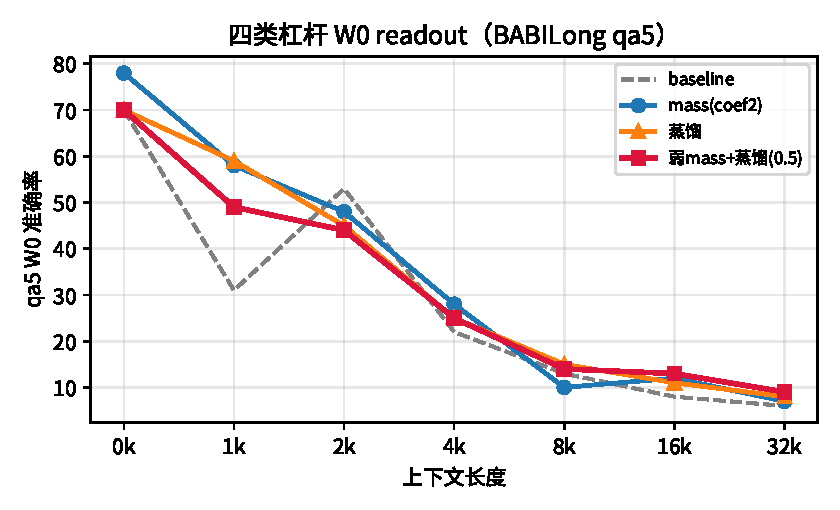
\includegraphics[width=0.82\textwidth]{figs/levers_qa5.pdf}
  \caption{四类杠杆在 BABILong qa5（chunk512，W0）各长度上的对比。}
\end{figure}
\noindent
（1）mass 与蒸馏各自有效：mass 在中短程把 qa5 翻倍（1k 31$\to$58）且 seed 鲁棒；蒸馏可复现、8k 处最强（15）。
（2）长度课程救回了“直训 32k 退化”，但未突破中程天花板。
（3）\textbf{【最重要】}：弱 mass（coef $\approx0.5$）+ 蒸馏在长程产生协同——下图显示随 mass 强度呈倒 U，峰值 coef $\approx0.5$ 时
16k=13、32k=9，首次超过所有单独方法；mass 过强（coef=2.0）则与蒸馏目标冲突、长程崩到 5--6。

\begin{figure}[H]\centering
  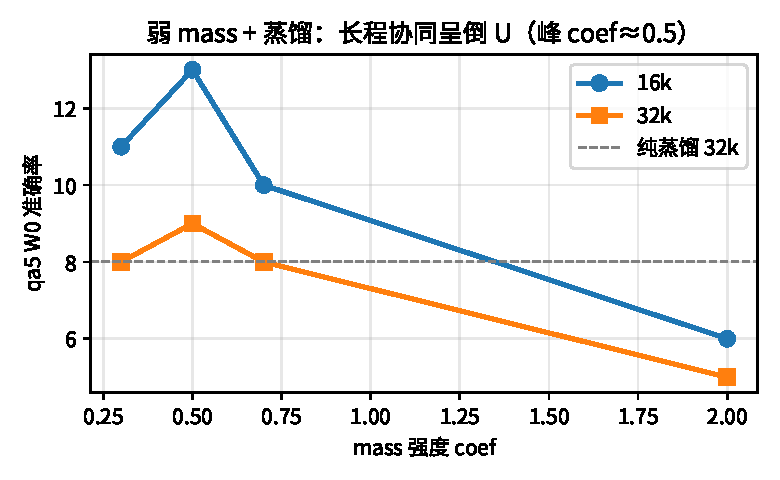
\includegraphics[width=0.72\textwidth]{figs/coef_invertedU.pdf}
  \caption{弱叠加 coef 精扫：长程 qa5 随 mass 强度呈倒 U，峰值在 coef$\approx$0.5。}
\end{figure}
\noindent
（4）长训退化：最优配置在约 500 步即收敛，继续训到 1000 步长程反而下降（32k 9$\to$6）——“早停”是甜点，不应盲目加训练量。

\subsection{LongBench 真实长文档：能力缺失定位}
\begin{figure}[H]\centering
  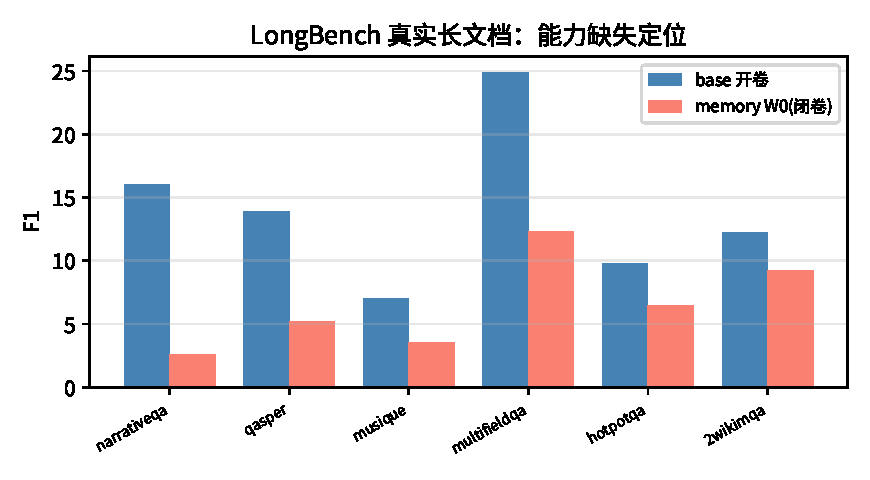
\includegraphics[width=0.86\textwidth]{figs/longbench_gap.pdf}
  \caption{LongBench 6 数据集：记忆模型 W0（F1）相对 base 开卷基线的保留率。}
\end{figure}
\noindent
我们首次在真实长文档 QA（LongBench 6 数据集）上拿到记忆模型的 W0 分（此前因显存竞争与格式问题屡次静默失败）。
对照 base 模型开卷基线，能力缺失高度集中：narrativeqa（超长叙事）几乎全失效（16.0$\to$2.6，仅保留 16\%），
qasper（科学论文细节）保留 38\%；而多跳检索类（2wikimqa/hotpotqa）保留 66--75\% 相对最好——
恰是合成检索训练强化的“跨片段关联”能力。这把下一步要攻的短板明确指向
“超长单一文档的连贯保持”与“细粒度信息保真”，而非关联检索。

% ================= 4 工程护栏 =================
\section{工程实践与质量护栏}
大模型驱动的高强度实验会遇到大量“看着在跑、其实没效果”的静默失效。本工作把每次踩坑都沉淀为代码级护栏，
形成质量闭环——这是“大模型驱动软件开发”能否可靠的关键：
\begin{itemize}
  \item \textbf{数据饥饿 $\to$ 启动即报错}：dolmino 单文档上限 4096 token，当 $(n\_ctx+1)\times$chunk\_size 超限时 loader 零产出、
        DDP 第一步静默死锁。修复：零产出 epoch 直接 raise，并把长度课程解耦到 T2 流（dolmino 锁 n\_ctx=3）。
  \item \textbf{蒸馏缓存失配 $\to$ 指纹断言 + 命中率 fail-fast}：teacher 缓存按位置索引，跨盘数据集行序不同 / 文件漏同步会导致
        100\% cache miss、蒸馏静默失效。修复：缓存记录数据集 fingerprint，训练启动断言一致；step50 命中率为 0 即 raise。
  \item \textbf{NCCL teardown 僵死}：训练逻辑完成却卡在 teardown，busy=8/8 假象占卡数小时。巡检需交叉验证进程状态与 final ckpt。
  \item \textbf{显存竞争 OOM}：启动训练前必须查 nvidia-smi 真实显存（不能只看 proc 数），避免与残留进程争抢。
  \item \textbf{跨盘一致性}：三个独立物理盘（diskA/diskB/B200-wzc1），代码改动需完整 rsync（含 build/launch/src 全部文件）。
  \item \textbf{LongBench chat\_template}：base 模型无 chat\_template，脚本硬编码 \texttt{--use\_chat\_template} 致全 worker 首样本崩溃；改为默认关闭。
\end{itemize}
这些护栏的共同主题是：把静默失效转化为快速、显式的失败，让 Agent 在下一个巡检周期就能发现并自愈，
而不是浪费数小时算力。

% ================= 5 结论 =================
\section{结论与展望}
\begin{itemize}
  \item MoM 的 MoE 式 top-$k$ 路由能在有界 KV 下承载长上下文，但读写解耦带来“读不准”的核心瓶颈。
  \item 机制侧杠杆（mass、蒸馏）优于训练侧（容量/长度/课程）；弱 mass+蒸馏的组合在长程首次超过单独方法。
  \item 长程 32k 仍是共同天花板（6$\to$9），未被根本突破；真实长文档上缺失集中于超长叙事与细粒度抽取。
  \item 展望：沿最优弱叠加配置 + 针对“连贯/细粒度”的新机制，配合 LongBench 持续验证。
\end{itemize}
方法论层面，本工作验证了大模型 Agent 可以自主驱动一个真实的多节点 ML 研究项目——
从调度到排错到结论——并通过护栏沉淀保证工程可靠性。

% ================= 附录 =================
\appendix
\newpage
\section{完整 W0 对照表（BABILong qa5，chunk512，0--32k）}
\begin{center}\small
\begin{tabular}{lccccccc}
\toprule
\textbf{配置} & \textbf{0k} & \textbf{1k} & \textbf{2k} & \textbf{4k} & \textbf{8k} & \textbf{16k} & \textbf{32k}\\
\midrule
baseline (T2\_chunk512) & 70 & 31 & 53 & 22 & 13 & 8 & 6\\
mass coef0.5 & 73 & 49 & 40 & 25 & 10 & 12 & 9\\
mass coef2.0 & 78 & 58 & 48 & 28 & 10 & 12 & 7\\
mass coef2 (seed1234) & 63 & 58 & 46 & 26 & 12 & 10 & 8\\
蒸馏 A+B & 70 & 59 & 45 & 25 & 15 & 11 & 8\\
叠加 coef0.5+蒸馏 & 70 & 49 & 44 & 25 & 14 & \textbf{13} & \textbf{9}\\
叠加 coef0.7+蒸馏 & 69 & 57 & 36 & 26 & 11 & 10 & 8\\
叠加 coef2.0+蒸馏 & 71 & 50 & 33 & 22 & 10 & 6 & 5\\
\bottomrule
\end{tabular}
\end{center}

\section{弱叠加 coef 精扫（长程 qa5）}
\begin{center}
\begin{tabular}{cccc}
\toprule
\textbf{coef} & \textbf{8k} & \textbf{16k} & \textbf{32k}\\
\midrule
0.3 & 14 & 11 & 8\\
0.5 & 14 & \textbf{13} & \textbf{9}\\
0.7 & 11 & 10 & 8\\
2.0 & 10 & 6 & 5\\
\bottomrule
\end{tabular}
\end{center}

\section{LongBench W0（F1）vs base 开卷基线}
\begin{center}
\begin{tabular}{lccc}
\toprule
\textbf{数据集} & \textbf{mem W0} & \textbf{base 开卷} & \textbf{保留率}\\
\midrule
narrativeqa & 2.6 & 16.0 & 16\%\\
qasper & 5.2 & 13.9 & 38\%\\
musique & 3.5 & 7.0 & 50\%\\
multifieldqa\_en & 12.3 & 24.9 & 49\%\\
hotpotqa & 6.5 & 9.8 & 66\%\\
2wikimqa & 9.2 & 12.2 & 75\%\\
\midrule
\textbf{平均} & \textbf{6.56} & \textbf{14.0} & \textbf{47\%}\\
\bottomrule
\end{tabular}
\end{center}

\section{关键代码与脚本}
\begin{itemize}
  \item 架构：\texttt{src/memory/mem\_space/\{config,layer,selector,memory\_bank,l3\_summary\}.py}
  \item token-mass：\texttt{--use\_readout\_mass\_bias --readout\_mass\_coef}（commit 79ad265）
  \item self-study 蒸馏：\texttt{scripts/build\_distill\_cache.py} + \texttt{scripts/launch\_distill\_chunk512\_AB.sh}（commit 19477fb / 8ea2969）
  \item 长度课程解耦 + 数据饥饿护栏：\texttt{--t2\_curriculum}（commit dadc19f / 2c22d80）
  \item 缓存指纹 + 命中率 fail-fast：commit 0cf2c23 / 438b674
  \item 设计文档：\texttt{versions/v21\_selfstudy\_distillation.md}
  \item 阶段报告：\texttt{status/READOUT\_ATTACK\_STAGING\_REPORT.md}
  \item 源码仓库：\url{https://github.com/liuhanzuo/Mixture-of-Memory}
\end{itemize}

\end{document}
